\chapter{Evaluaci\'on del programa original}
\label{ch:prev_work}

A continuaci\'on se exponen los resultados de diferentes pruebas realizadas sobre el programa original con la finalidad de medir su desempe\~no computacional en t\'erminos de tiempo de ejecuci\'on y uso de memoria.
\bigskip

Estas pruebas se llevaron a cabo en un computador personal de 8 GB (DDR4) de RAM. La raz\'on de esta  medida (que no se hayan ejecutado en Leftraru) es que el c\'odigo original contiene demasiadas l\'ineas con el comando \texttt{glob}\footnote{\url{https://docs.python.org/3.5/library/glob.html}} de Python el cual lista reiteradamente el contenido de los directorios de los archivos lo que finalmente termina saturando el nodo destinado para el lanzamiento del programa (ya que recorre la lista de 93 supernovas de HiTS, repitiendo para cada una de ellas el mismo proceso). Por esta raz\'on, los administradores del sistema del NLHPC sugirieron modificaciones al programa original, sin embargo, en pos de continuar con el esp\'iritu de esta tesis, se opt\'o por efectuar los experimentos de manera local (usando un computador personal) evitando as\'i introducir m\'as modificaciones (se adapt\'o el programa para Python 3.6, ya que originalmente estaba para 2.7 agregando cambios menores como la forma de imprimir mensajes en consola (\texttt{print})).
\bigskip

La pipeline original (\texttt{candidate\_search}) est\'a estructurada, a grandes rasgos por dos bloques de \textbf{detecci\'on}: el primero est\'a destinado a buscar una supernova confirmada por HiTS (cuya coordenada es conocida) y el segundo a obtener la informaci\'on de otros posibles candidatos que se hayan encontrado anteriormente. Cabe recalcar que a este segundo proceso se ingresa s\'olo en el caso que se hayan encontrado candidatos desconocidos en primera fase.
\bigskip

El proceso de b\'usqueda de la supernova se inicializa en una instancia de \textsc{RunData}, \textbf{listando los archivos desde disco}, para preparar las im\'agenes y el resto de archivos que ser\'an usados para el proceso iterativo que se lista a continuaci\'on: 

\begin{enumerate}
\item \textbf{C\'alculo de flujo:} A partir de las im\'agenes cient\'ificas y de calibraci\'on se obtiene el flujo (en ADU\footnote{Analog-to-digital unit}) por pixel y es registrado en una matriz (\texttt{numpy array}) en cada iteraci\'on. 
\item \textbf{Proceso de estimaci\'on con filtro de Kalman:} En este paso se realizan los procesos de predicci\'on y correcci\'on para obtener una nueva estimaci\'on. 
\item \textbf{Detecci\'on de fuentes:} En este paso se estudia la idoneidad de los pixeles tanto del flujo como de las estimaciones de los mismos (obtenidos con el filtro de Kalman) y del resto de las im\'agenes al momento de verificar una serie de criterios con los cuales estos se agrupar\'ian entre vecinos para formar potenciales candidatos.  
\item \textbf{Actualizaci\'on de candidatos:} Revisa si hay nuevos candidatos a ser considerados. Se registran en un arreglo (\texttt{numpy array}).
\end{enumerate}

Si en el proceso anterior se encuentra alg\'un candidato, se procede a repetir los pasos de obtenci\'on de flujos, estimaciones y filtrado de pixeles. La diferencia est\'a en que en esta ocasi\'on se van guardando los resultados en una estructura de datos de diccionario. El nuevo ciclo queda como sigue:

\begin{enumerate}

\item \textbf{Repetici\'on de los pasos anteriores 1-3}
\item \textbf{Guardado de resultados:} La informaci\'on de los nuevos candidatos encontrados previamente es guardado en una estructura de diccionario y registrado en disco usando el formato NPZ (formato brindado por \textsc{Numpy} para comprimir datos).
\end{enumerate}


El diagrama de la Figura \ref{fig:des_sif} entrega una perspectiva general de la secuencia de pasos que realiza el programa.
\bigskip

Cabe destacar que durante el proceso de refactoring del programa original se encontr\'o que la lista de archivos, que debe ser procesada en orden de acuerdo a la \'epoca (o fecha de observaci\'on) no estaba siendo bien ordenada durante el proceso de selecci\'on de im\'agenes cient\'ificas a partir del valor de \texttt{airmass} en la clase \textsc{FitsHandler}.
\bigskip


\begin{figure}[h!]
\centering
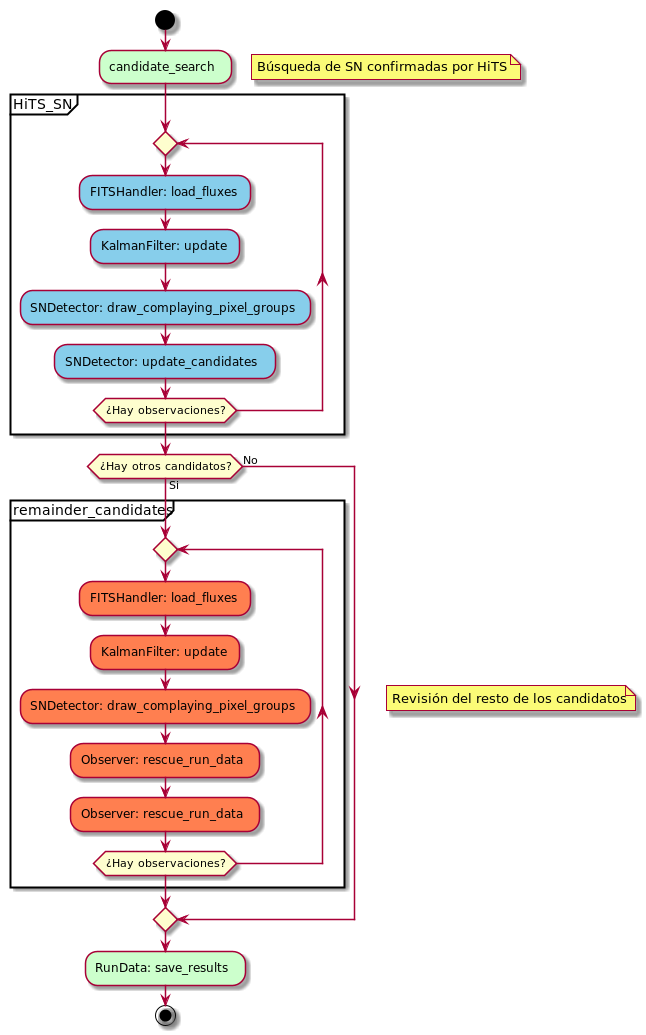
\includegraphics[scale=.5]{images/results/sif_act}
\caption{Diagrama de flujo del programa original. Se aprec\'ian dos ciclos principales: el primero est\'a destinado a la b\'usqueda de una supernova de HiTS, y el segundo a la revisi\'on de la lista de posibles candidatos encontrados durante la verificaci\'on de la supernova de HiTS. Notar que hay pasos que se repiten en la realizaci\'on de ambos an\'alisis.}
\label{fig:des_sif}
\end{figure}

\section{Estructura de datos}
\label{des:struct}
Debido a la naturaleza de la informaci\'on de entrada (im\'agenes) se debe trabajar en p\'ixeles, por lo que la estructura de datos que representen las variables de estado debe considerar la dimensi\'on de las im\'agenes (considerando que por cada p\'ixel se debe modelar las variables de estado flujo y velocidad de flujo, y covarianza asociada). Debido a esto, en el trabajo de Pablo Huentelemu \cite{huentelemu} se dise\~naron \textit{hiperrect\'angulos} para modelar las variables de estado y covarianza de todos los pixeles de una imagen. Los datasets contienen im\'agenes de dimensi\'on  $2046 \times 4096$. La figura \ref{fig:data_scheme} muestra el esquema de sistema de matrices o \textit{hiperrect\'angulos} usada para representar el estado de cada p\'ixel y su recpectiva covarianza.
\bigskip  

\begin{figure}
\centering
\includegraphics[scale=.35]{/home/paloma/Documents/Memoria/SVG/hola.png}
\caption{Esquema las estructuras de datos usadas para la representaci\'on de las matrices de estados y de las matrices de covarianza de la relaci\'on entre el flujo y la velocidad de flujo para cada pixel, de una imagen de ancho $w$ y altura $h$. Para los conjuntos de datos, $w=2046$ y $h=4096$.}
\label{fig:data_scheme}
\end{figure}
\bigskip

\section{Tiempo de ejecuci\'on}

El estudio del tiempo de ejecuci\'on del programa se realiz\'o usando la funci\'on \texttt{getrusage} de la librer\'ia \texttt{resource} de Python, midiendo el tiempo de usuario en segundos. Las mediciones se realizaron sobre tres conjuntos de datos (las cuales contienen alguna supernova detectada por HiTS) seleccionados al azar: SN14, SN18 y  SN80. En cada uno de ellos comprende secuencias de 26, 23 y 18 observaciones respectivamente. 
\bigskip

Las tablas \ref{tab:t1} y \ref{tab:t2} muestran el tiempo en segundos que toma el proceso de detecci\'on de candidatos. Se destacan como procesos separados el reconocimiento de la supernova de HiTS y posteriormente, el proceso de estudio de los nuevos candidatos, respectivamente, empleando para ambos procesos el filtro B\'asico.  

\begin{table}[h!]
\centering
\caption{Resultados de tiempos de ejecuci\'on correspondientes a calculo de flujos, estimaci\'on de los filtros, agrupaci\'on de pixeles y filtrado de los mismos durante el per\'iodo de reconocimiento de la supernova correspondiente. Para esta prueba se utiliz\'o el filtro de Kalman B\'asico. La \'ultima fila corresponde a la media por observaci\'on.}
\begin{tabular}{|l|l|l|l|l|}
\hline
\textbf{ID} & \textbf{C\'alc. Flujos [s]} & \textbf{Aplic. KF [s]} &  \textbf{Agrup. Pixeles [s]}  & \textbf{Actual. Candidatos [s]}\\ \hline \hline
SN14        & 293.91            & 24.90        &  68.30 & 0.02 \\ \hline
SN18            & 260.09             & 22.56         &  45.52  & 0.00\\ \hline
SN80            & 204.93             & 17.69         &   38.21 & 0.00 \\ \hline \hline
%Media & 303.08 &  26.23 & 37.83 & 0.01\\\hline 
$\bar{t}/Obs$ & 11.00 &  0.97 & 2.24 & 0.00\\\hline 
\end{tabular}
\label{tab:t1}
\end{table}

\begin{table}[h!]
\centering
\caption{Resultados de tiempos de ejecuci\'on correspondientes a calculo de flujos, estimaci\'on de los filtros, agrupaci\'on de pixeles y filtrado de los mismos durante el peri\'odo de estudio de los nuevos candidatos encontrados en el paso anterior. Para esta prueba se utiliz\'o el filtro de Kalman B\'asico. Se observa que para las dos \'ultimas supernovas los tiempos son cero ya que no se encontraron m\'as candidatos.}
\begin{tabular}{|l|l|l|l|l|}
\hline
\textbf{ID} & \textbf{C\'alc. Flujos [s]} & \textbf{Aplic. KF [s]} &  \textbf{Agrup. Pixeles [s]}  & \textbf{Guardar resultados [s]}\\ \hline \hline
SN14        & 303.18            & 27.28        &  72.34 & 0.02 \\ \hline
SN18            & 0.00             & 0.00         &  0.00  & 0.00\\ \hline
SN80            & 0.00             & 0.00         &   0.00 & 0.00 \\ \hline\hline 
%Media & 306.98 &  28.89 & 38.89  & 0.07\\\hline 
$\bar{t}/Obs$ & 11.66 &  1.05 & 2.78 & 0.00\\\hline 
\end{tabular}
\label{tab:t2}
\end{table}

Las tablas \ref{tab:t3} y el \ref{tab:t4} describen el tiempo (en segundos) tomado tanto para el proceso de detecci\'on de la supernova de HiTS y el posterior procesamiento de posibles nuevos candidatos (en ese orden) usando el filtro de m\'axima correntrop\'ia.
\bigskip
 
\begin{table}[h!]
\centering
\caption{Resultados de tiempos de ejecuci\'on correspondientes a calculo de flujos, estimaci\'on de los filtros, agrupaci\'on de pixeles y filtrado de los mismos durante el per\'iodo de reconocimiento de la supernova correspondiente. Para esta prueba se utiliz\'o el filtro de Kalman de M\'axima Correntrop\'ia.}
\begin{tabular}{|l|l|l|l|l|}
\hline
\textbf{ID} & \textbf{C\'alc. Flujos [s]} & \textbf{Aplic. KF [s]} &  \textbf{Agrup. Pixeles [s]}  & \textbf{Actual. Candidatos [s]}\\ \hline \hline
SN14        & 342.44            & 798.48        &  76.47 & 0.00 \\ \hline
SN18            & 273.64             & 566.89         &  47.96  & 0.00\\ \hline
SN80            & 210.68             & 420.12         &   36.05 & 0.00 \\ \hline \hline 
%Media & 309.32 & 638.48 &  37.07 & 0.01\\\hline
$\bar{t}/Obs. $& 12.25 & 26.23 & 2.34 & 0.00\\\hline 
\end{tabular}
\label{tab:t3}
\end{table}

\begin{table}[h!]
\centering
\caption{Resultados de tiempos de ejecuci\'on correspondientes a calculo de flujos, estimaci\'on de los filtros, agrupaci\'on de pixeles y filtrado de los mismos durante el per\'iodo de estudio de los nuevos candidatos encontrados en el paso anterior. Para esta prueba se utiliz\'o el filtro de Kalman de M\'axima Correntrop\'ia. Se observa que para las dos \'ultimas supernovas los tiempos son cero ya que no se encontraron m\'as candidatos.}
\begin{tabular}{|l|l|l|l|l|}
\hline
\textbf{ID} & \textbf{C\'alc. Flujos [s]} & \textbf{Aplic. KF [s]} &  \textbf{Agrup. Pixeles [s]}  & \textbf{Guardar resultados [s]}\\ \hline \hline
SN14        & 307.64            & 680.65        &  65.67 & 0.02 \\ \hline
SN18            & 0.00             & 0.00         &  0.00  & 0.00\\ \hline
SN80            & 0.00             & 0.00         &   0.00 & 0.00 \\ \hline \hline
%Media & 306.71 & 634.09 &  36.34 & 0.05\\\hline
$\bar{t}/Obs. $& 11.83 & 26.18 & 2.53 & 0.00\\\hline  
\end{tabular}
\label{tab:t4}

\end{table}
\bigskip

La tabla \ref{tab:t5} muestra el tiempo total comprendido por ambos subprocesos usando el filtro de Kalman B\'asico. Se destaca la diferencia del consumo de tiempo ante la ausencia y presencia de nuevos candidatos a supernova. Por otro lado, la tabla \ref{tab:t6} muestran las mismas medidas de tiempo para el filtro de m\'axima correntrop\'ia. Se destaca el aumento considerable de tiempo al usar este \'ultimo filtro en relaci\'on al primero. 
  
\begin{table}[h!]
\centering
\caption{Tiempo de ejecuci\'on de los procesos de b\'usqueda de supernova de HiTS, revisi\'on de los candidatos encontrados y tiempo total comprendido por ambos procesos usando filtro de Kalman B\'asico. La \'ultima fila corresponde a tiempo total promedio por observaci\'on.}
\begin{tabular}{|l|l|l|l|}
\hline
\textbf{ID} & \textbf{B\'usqueda SN [s]} & \textbf{Revisi\'on candidatos[s]} & \textbf{Tiempo total [s]} \\ \hline
\hline
SN14 & 387.13 & 402.82 & 789.95 \\\hline
SN18 & 328.17 & 0.00 & 328.17\\\hline
SN80 & 260.83 & 0.00 & 260.83 \\\hline\hline
%Media & 367.15 & 374.83 & 741.98  \\\hline
 $\bar{t}/Obs. $& 14.55 & -- & --\\\hline 
\end{tabular}
\label{tab:t5}
\end{table}


\begin{table}[h!]
\centering
\caption{Tiempo de ejecuci\'on de los procesos de b\'usqueda de supernova de HiTS, revisi\'on de los candidatos encontrados y tiempo total comprendido por ambos procesos usando filtro de Kalman de M\'axima correntrop\'ia.}
\begin{tabular}{|l|l|l|l|}
\hline
\textbf{ID} & \textbf{B\'usqueda SN [s]} & \textbf{Revisi\'on candidatos [s]} & \textbf{Tiempo total [s]} \\ \hline
\hline
SN14 & 1217.39 & 1053.98 & 2068.80\\\hline
SN18 & 888.49 & 0.00 & 0.00\\\hline
SN80 & 666.85 & 0.00& 0.00\\\hline \hline
 $\bar{t}/Obs. $& 40.83 & -- & --\\\hline 
\end{tabular}
\label{tab:t6}
\end{table}

\section{Uso de memoria}

La memoria ocupada por el programa se midi\'o en t\'erminos de MiB (Mebibyte) usando la librer\'ia \texttt{memory\_profiler}. Posteriormente las mediciones en la unidad previamente mencionada fueron pasadas a MB\footnote{$1MiB\simeq 1.049MB$ }.
\bigskip

La figura \ref{fig:mem_kbf} muestra el comportamiento del uso de memoria principal (en t\'erminos de Mebibytes) para los tres conjuntos de datos empleados, usando el filtro de Kalman B\'asico. Se distinguen un uso m\'as intensivo (m\'aximo alcanzado) durante el proceso en que se usaron los datos de la SN14, la cual no s\'olo posee una secuencia de im\'agenes mayor (de 26) sino tambi\'en corresponde a aquella en donde se encontraron posibles nuevos candidatos. En la tabla \ref{tab:mem1} se expone el m\'aximo consumo generado durante la ejecuci\'on de la pipeline empleando el filtro B\'asico.
\bigskip

\begin{figure}[h!]
\centering
\subfloat[Memoria ocupada en SN14]{\label{fig:kbf_14}{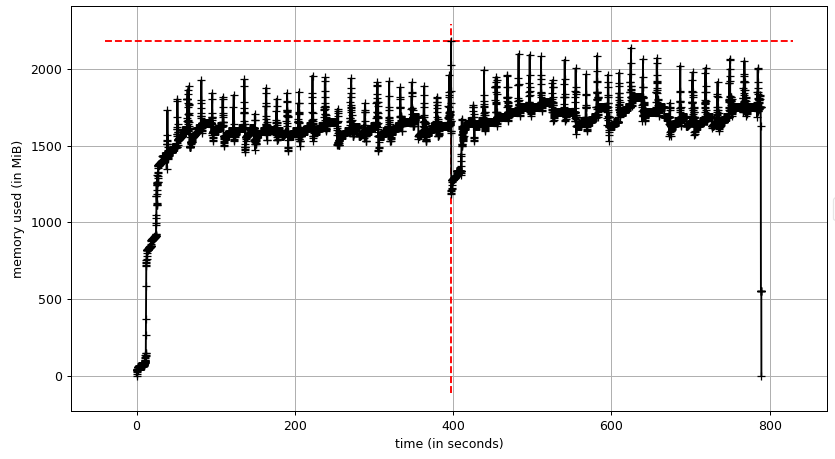
\includegraphics[width=0.5\textwidth]{images/results/sn14_00}}}\hfill
\subfloat[Memoria ocupada en SN18]{\label{fig:kbf_18}{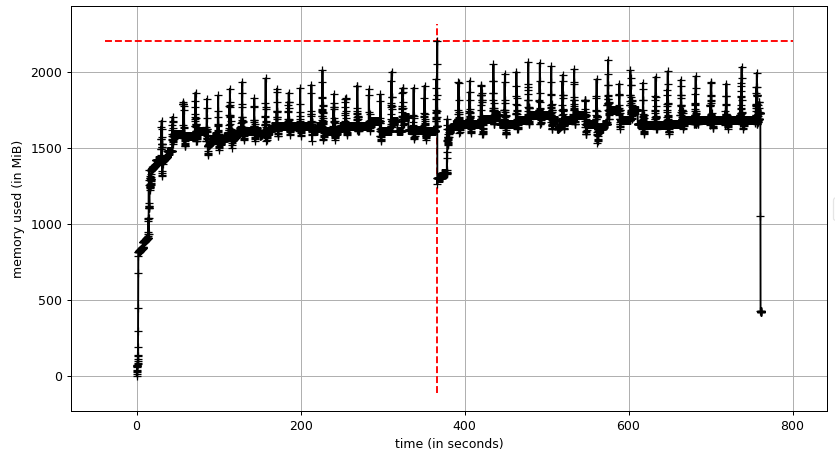
\includegraphics[width=0.5\textwidth]{images/results/sn18_00}}}\vfill
\subfloat[Memoria ocupada en SN80]{\label{fig:kbf_80}{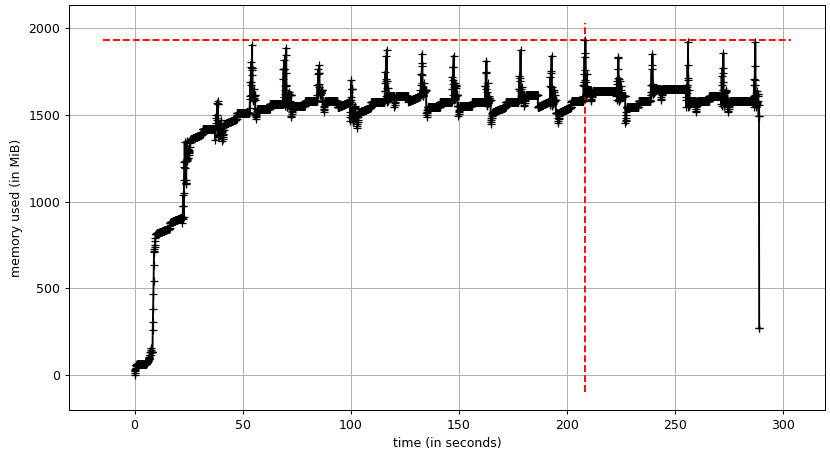
\includegraphics[width=0.5\textwidth]{images/results/sn80_00}}}
\caption{Comportamiento de la memoria (en mebibytes) durante la ejecuci\'on para los tres conjuntos de datos usando el filtro de Kalman B\'asico.}
\label{fig:mem_kbf}
\end{figure}

 
\begin{table}[h!]
\centering
\caption{Memoria principal (en unidades de MB) usada durante la ejecuci\'on del programa original usando la versi\'on b\'asica del filtro de Kalman.}
\begin{tabular}{|l|l|}
\hline
\textbf{ID} & Memoria [MB]\\\hline\hline
SN14 & 2282.42\\\hline
SN18 & 2063.02\\\hline
SN80 & 2021.27\\\hline
\end{tabular}

\label{tab:mem1}
\end{table}


La figura \ref{fig:mem_mcc} muestra el consumo de memoria (en Mebibytes) para la ejecuci\'on del programa original para los tres conjuntos de datos, usando el filtro de m\'axima correntrop\'ia. Se destaca un comportamiento similar al obtenido usando el filtro b\'asico debido a  la detecci\'on de posibles candidatos con el conjunto de datos de la SN14. Por otro lado, se desprende un mayor consumo de parte de este filtro en relaci\'on a la versi\'on b\'asica. La tabla \ref{tab:mem2} describe el consumo m\'aximo de memoria alcanzado con el uso del filtro de m\'axima correntrop\'ia.
\bigskip

\begin{figure}[h!]
\centering
\subfloat[Memoria ocupada en SN14]{\label{fig:mc_14}{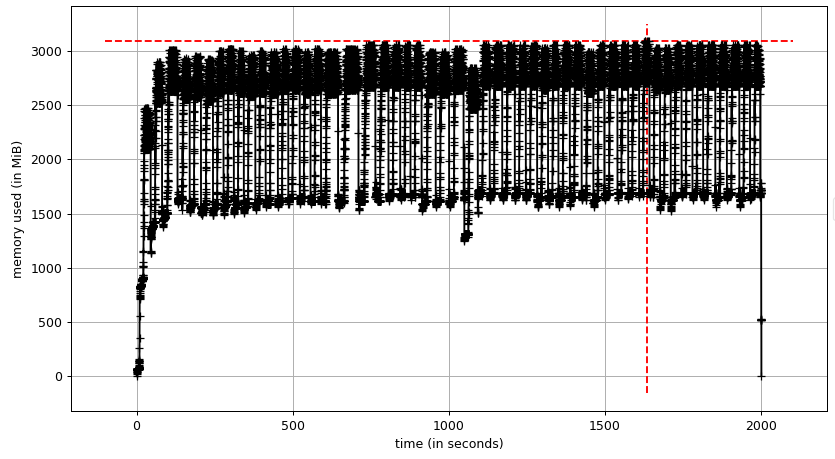
\includegraphics[width=0.5\textwidth]{images/results/sn14_01}}}\hfill
\subfloat[Memoria ocupada en SN18]{\label{fig:mc_18}{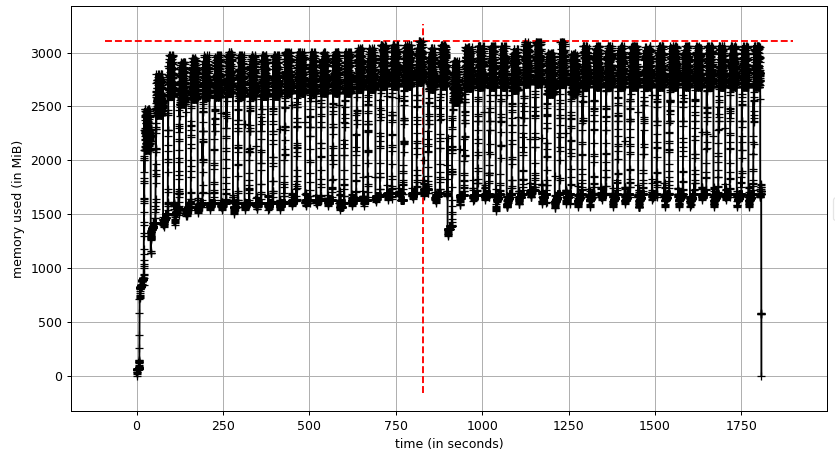
\includegraphics[width=0.5\textwidth]{images/results/sn18_01}}}\vfill
\subfloat[Memoria ocupada en SN80]{\label{fig:mc_80}{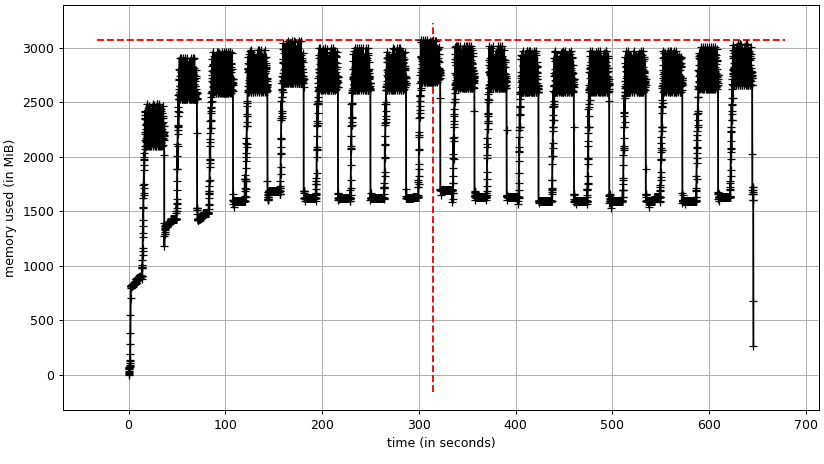
\includegraphics[width=0.5\textwidth]{images/results/sn80_01}}}
\caption{Comportamiento de la memoria (en mebibytes) durante la ejecuci\'on para los tres conjuntos de datos. En los tres lanzamientos se us\'o el filtro de Kalman de correntrop\'ia m\'axima.}
\label{fig:mem_mcc}
\end{figure}


\begin{table}[h!]
\centering
\caption{Memoria principal (en unidades de MB) usada durante la ejecuci\'on del programa original usando filtro de Kalman de m\'axima correntrop\'ia.}
\begin{tabular}{|l|l|}
\hline
\textbf{ID} & Memoria [MB]\\\hline\hline
SN14 & 3353.13\\\hline
SN18 & 3194.96\\\hline
SN80 & 3209.67\\\hline
\end{tabular}
\label{tab:mem2}
\end{table}

\section{Falsos negativos y verdaderos positivos}
La Tabla \ref{tab:tpfn}, muestra el resultado de la detecci\'on de las 93 supernovas de HiTS para el conjunto de datos del a\~no 2015. Se logr\'o realizar las pruebas en Leftraru durante el mes de diciembre de 2018 liberando memoria (evitando as\'i problemas asociados al enlistado de archivos usando \texttt{glob}).
\bigskip

\begin{table}[h!]
\centering
\caption{N\'umero de falsos negativos (FN) y verdaderos positivos (TP) encontrados usando cada uno de los filtros. La tercera columna, \textbf{NaN} indica el n\'umero conjunto de datos que no se pudieron procesar por falta de alguna informaci\'on de entrada. No se observan diferencias sustanciales entre los resultados de cada filtro.}
\begin{tabular}{|l|l|l|l|}
\hline
\textbf{Filtro} & \textbf{TP} & \textbf{FN} & \textbf{NaN}\\ \hline
Básico          & 33          & 57         & 3 \\ \hline
MCC             & 33          & 57         & 3 \\ \hline
\end{tabular}
\label{tab:tpfn}
\end{table}

Estableciendo par\'ametros de umbral de 200.0 para flujo y de 50.0 para la velocidad de flujo (cantidades estimadas para el filtro de Kalman) se obtienen resultados id\'enticos para ambos filtros al momento de detectar supernovas conocidas por HiTS. En ambos casos se detectaron 33 de 90, ya que para tres supernovas (de las 93 y \'ultimas en la lista) no se encontraron las im\'agenes de invarianza inversa.
\bigskip

Sin embargo, cabe destacar que dentro de las 93 supernovas, existen 36 (las primeras de la lista) de las cuales se conoce que corresponden a supernovas j\'ovenes que se encuentran en pleno per\'iodo de aumento de luminosidad. De estas 36, para ambos filtros, se detectaron 22 lo que corresponder\'ia a un 61\%. El descarte de pixeles genera la disminuci\'on de puntos a considerar en la estimaci\'on de la curva lo que perjudica al filtro en la toma de decisi\'on al requerir al menos 5 a 6 puntos (mediciones) consecutivos. Por esta raz\'on se piensa que el desarrollo de un nuevo filtro de aproximaci\'on no-lineal podr\'ia mejorar este resultado.
\bigskip

\subsection{\'Epocas de detecci\'on}

Al estudiar los periodos de las detecciones de cada uno de los conjuntos de datos de las supernovas de HiTS, para ambos filtros, se obtiene que no hay diferencias en la \'epoca en que se realiza (es decir misma hora o MJD). Ver Ap\'endice, secci\'on \ref{ap:tab1}. 
\bigskip

Las Im\'agenes \ref{fig:orig_det_snL} y \ref{fig:orig_det_snaa} muestran dos casos del int\'ervalo de tiempo en que se realiza la detecci\'on usando las implementaciones de los filtros del programa original.
\bigskip

\begin{figure}[h!]
\centering
\includegraphics[scale=0.35]{/home/paloma/Documents/Memoria/SVG/hits_snL.png}
\caption{Curva de luz (en ADU (\textit{analog-to-digital unit}) vs MJD) de supernova  observada durante el periodo del primer semestre del 2015 cuyo registro se realiz\'o en el CCD N27, en el campo 34. La detecci\'on realizada por los filtros b\'asico y de m\'axima correntrop\'ia se realiz\'o en el MJD 57072.214 (\'epoca u observaci\'on 7 de 18). }
\label{fig:orig_det_snL}
\end{figure}

La Figura \ref{fig:orig_det_snL} muestra una detecci\'on dentro de un claro regimen creciente, que puede ser observado casi al comienzo de la curva de luz (\'epoca 7 de 18). La figura \ref{fig:orig_det_snaa}, por el contrario, muestra una detecci\'on (realizada en la \'epoca 23 de 27) en un r\'egimen no muy claro y de bastante ruido.


\begin{figure}[h!]
\centering
\includegraphics[scale=0.35]{/home/paloma/Documents/Memoria/SVG/hits_snaa.png}
\caption{Curva de luz supernova observada durante el periodo del primer semestre del 2015 cuyo registro se realiz\'o en el CCD S5, en el campo 21. Ambos filtros detectaron la supernova en el MJD 57077.166 (\'epoca u observaci\'on 23 de 27).}
\label{fig:orig_det_snaa}
\end{figure}
\bigskip

\section{Falsos positivos}
El poder reconocer falsos positivos a trav\'es de este algoritmo se hace imposible si no se cuenta con una herramienta externa de visualizaci\'on o de machine learning (por ejemplo, usando un clasificador de conjuntos de pixeles que eval\'ue la probabilidad de que se trata efectivamente de una supernova joven). Esto se debe a que existen variados objetos como estrellas variables o \textit{artefactos} que corresponden a zonas ruidosas de la imagen  cient\'ifica (en particular, bordes) y pueden proveer valores alterados de flujo lo que en algunos casos puede conllevar a la detecci\'on de falsos positivos.
\bigskip

Una forma de poder estudiar un falso positivo es a trav\'es de la visualizaci\'on de su espacio de fase y la obtenci\'on de su curva entr\'opica.